\documentclass[10pt, conference, compsocconf]{IEEEtran}

% *** GRAPHICS RELATED PACKAGES ***
%
\ifCLASSINFOpdf
  \usepackage[pdftex]{graphicx}
  % declare the path(s) where your graphic files are
  % \graphicspath{{../pdf/}{../jpeg/}}
  % and their extensions so you won't have to specify these with
  % every instance of \includegraphics
  % \DeclareGraphicsExtensions{.pdf,.jpeg,.png}
\else
  % or other class option (dvipsone, dvipdf, if not using dvips). graphicx
  % will default to the driver specified in the system graphics.cfg if no
  % driver is specified.
  % \usepackage[dvips]{graphicx}
  % declare the path(s) where your graphic files are
  % \graphicspath{{../eps/}}
  % and their extensions so you won't have to specify these with
  % every instance of \includegraphics
  % \DeclareGraphicsExtensions{.eps}
\fi
% graphicx was written by David Carlisle and Sebastian Rahtz. It is
% required if you want graphics, photos, etc. graphicx.sty is already
% installed on most LaTeX systems. The latest version and documentation can
% be obtained at: 
% http://www.ctan.org/tex-archive/macros/latex/required/graphics/
% Another good source of documentation is "Using Imported Graphics in
% LaTeX2e" by Keith Reckdahl which can be found as epslatex.ps or
% epslatex.pdf at: http://www.ctan.org/tex-archive/info/
%
% latex, and pdflatex in dvi mode, support graphics in encapsulated
% postscript (.eps) format. pdflatex in pdf mode supports graphics
% in .pdf, .jpeg, .png and .mps (metapost) formats. Users should ensure
% that all non-photo figures use a vector format (.eps, .pdf, .mps) and
% not a bitmapped formats (.jpeg, .png). IEEE frowns on bitmapped formats
% which can result in "jaggedy"/blurry rendering of lines and letters as
% well as large increases in file sizes.
%
% You can find documentation about the pdfTeX application at:
% http://www.tug.org/applications/pdftex

\graphicspath{{img/}}

% *** MATH PACKAGES ***
%
%\usepackage[cmex10]{amsmath}
% A popular package from the American Mathematical Society that provides
% many useful and powerful commands for dealing with mathematics. If using
% it, be sure to load this package with the cmex10 option to ensure that
% only type 1 fonts will utilized at all point sizes. Without this option,
% it is possible that some math symbols, particularly those within
% footnotes, will be rendered in bitmap form which will result in a
% document that can not be IEEE Xplore compliant!
%
% Also, note that the amsmath package sets \interdisplaylinepenalty to 10000
% thus preventing page breaks from occurring within multiline equations. Use:
%\interdisplaylinepenalty=2500
% after loading amsmath to restore such page breaks as IEEEtran.cls normally
% does. amsmath.sty is already installed on most LaTeX systems. The latest
% version and documentation can be obtained at:
% http://www.ctan.org/tex-archive/macros/latex/required/amslatex/math/





% *** SPECIALIZED LIST PACKAGES ***
%
%\usepackage{algorithmic}
% algorithmic.sty was written by Peter Williams and Rogerio Brito.
% This package provides an algorithmic environment fo describing algorithms.
% You can use the algorithmic environment in-text or within a figure
% environment to provide for a floating algorithm. Do NOT use the algorithm
% floating environment provided by algorithm.sty (by the same authors) or
% algorithm2e.sty (by Christophe Fiorio) as IEEE does not use dedicated
% algorithm float types and packages that provide these will not provide
% correct IEEE style captions. The latest version and documentation of
% algorithmic.sty can be obtained at:
% http://www.ctan.org/tex-archive/macros/latex/contrib/algorithms/
% There is also a support site at:
% http://algorithms.berlios.de/index.html
% Also of interest may be the (relatively newer and more customizable)
% algorithmicx.sty package by Szasz Janos:
% http://www.ctan.org/tex-archive/macros/latex/contrib/algorithmicx/




% *** ALIGNMENT PACKAGES ***
%
%\usepackage{array}
% Frank Mittelbach's and David Carlisle's array.sty patches and improves
% the standard LaTeX2e array and tabular environments to provide better
% appearance and additional user controls. As the default LaTeX2e table
% generation code is lacking to the point of almost being broken with
% respect to the quality of the end results, all users are strongly
% advised to use an enhanced (at the very least that provided by array.sty)
% set of table tools. array.sty is already installed on most systems. The
% latest version and documentation can be obtained at:
% http://www.ctan.org/tex-archive/macros/latex/required/tools/


%\usepackage{mdwmath}
%\usepackage{mdwtab}
% Also highly recommended is Mark Wooding's extremely powerful MDW tools,
% especially mdwmath.sty and mdwtab.sty which are used to format equations
% and tables, respectively. The MDWtools set is already installed on most
% LaTeX systems. The lastest version and documentation is available at:
% http://www.ctan.org/tex-archive/macros/latex/contrib/mdwtools/


% IEEEtran contains the IEEEeqnarray family of commands that can be used to
% generate multiline equations as well as matrices, tables, etc., of high
% quality.


%\usepackage{eqparbox}
% Also of notable interest is Scott Pakin's eqparbox package for creating
% (automatically sized) equal width boxes - aka "natural width parboxes".
% Available at:
% http://www.ctan.org/tex-archive/macros/latex/contrib/eqparbox/





% *** SUBFIGURE PACKAGES ***
%\usepackage[tight,footnotesize]{subfigure}
% subfigure.sty was written by Steven Douglas Cochran. This package makes it
% easy to put subfigures in your figures. e.g., "Figure 1a and 1b". For IEEE
% work, it is a good idea to load it with the tight package option to reduce
% the amount of white space around the subfigures. subfigure.sty is already
% installed on most LaTeX systems. The latest version and documentation can
% be obtained at:
% http://www.ctan.org/tex-archive/obsolete/macros/latex/contrib/subfigure/
% subfigure.sty has been superceeded by subfig.sty.



%\usepackage[caption=false]{caption}
%\usepackage[font=footnotesize]{subfig}
% subfig.sty, also written by Steven Douglas Cochran, is the modern
% replacement for subfigure.sty. However, subfig.sty requires and
% automatically loads Axel Sommerfeldt's caption.sty which will override
% IEEEtran.cls handling of captions and this will result in nonIEEE style
% figure/table captions. To prevent this problem, be sure and preload
% caption.sty with its "caption=false" package option. This is will preserve
% IEEEtran.cls handing of captions. Version 1.3 (2005/06/28) and later 
% (recommended due to many improvements over 1.2) of subfig.sty supports
% the caption=false option directly:
%\usepackage[caption=false,font=footnotesize]{subfig}
%
% The latest version and documentation can be obtained at:
% http://www.ctan.org/tex-archive/macros/latex/contrib/subfig/
% The latest version and documentation of caption.sty can be obtained at:
% http://www.ctan.org/tex-archive/macros/latex/contrib/caption/




% *** FLOAT PACKAGES ***
%
%\usepackage{fixltx2e}
% fixltx2e, the successor to the earlier fix2col.sty, was written by
% Frank Mittelbach and David Carlisle. This package corrects a few problems
% in the LaTeX2e kernel, the most notable of which is that in current
% LaTeX2e releases, the ordering of single and double column floats is not
% guaranteed to be preserved. Thus, an unpatched LaTeX2e can allow a
% single column figure to be placed prior to an earlier double column
% figure. The latest version and documentation can be found at:
% http://www.ctan.org/tex-archive/macros/latex/base/



%\usepackage{stfloats}
% stfloats.sty was written by Sigitas Tolusis. This package gives LaTeX2e
% the ability to do double column floats at the bottom of the page as well
% as the top. (e.g., "\begin{figure*}[!b]" is not normally possible in
% LaTeX2e). It also provides a command:
%\fnbelowfloat
% to enable the placement of footnotes below bottom floats (the standard
% LaTeX2e kernel puts them above bottom floats). This is an invasive package
% which rewrites many portions of the LaTeX2e float routines. It may not work
% with other packages that modify the LaTeX2e float routines. The latest
% version and documentation can be obtained at:
% http://www.ctan.org/tex-archive/macros/latex/contrib/sttools/
% Documentation is contained in the stfloats.sty comments as well as in the
% presfull.pdf file. Do not use the stfloats baselinefloat ability as IEEE
% does not allow \baselineskip to stretch. Authors submitting work to the
% IEEE should note that IEEE rarely uses double column equations and
% that authors should try to avoid such use. Do not be tempted to use the
% cuted.sty or midfloat.sty packages (also by Sigitas Tolusis) as IEEE does
% not format its papers in such ways.





% *** PDF, URL AND HYPERLINK PACKAGES ***
%
%\usepackage{url}
% url.sty was written by Donald Arseneau. It provides better support for
% handling and breaking URLs. url.sty is already installed on most LaTeX
% systems. The latest version can be obtained at:
% http://www.ctan.org/tex-archive/macros/latex/contrib/misc/
% Read the url.sty source comments for usage information. Basically,
% \url{my_url_here}.





% *** Do not adjust lengths that control margins, column widths, etc. ***
% *** Do not use packages that alter fonts (such as pslatex).         ***
% There should be no need to do such things with IEEEtran.cls V1.6 and later.
% (Unless specifically asked to do so by the journal or conference you plan
% to submit to, of course. )


% correct bad hyphenation here
\hyphenation{op-tical net-works semi-conduc-tor}
\usepackage[brazilian]{babel}
\usepackage[utf8]{inputenc}
\usepackage[T1]{fontenc}


\begin{document}
%
% paper title
% can use linebreaks \\ within to get better formatting as desired
\title{LSystem2Unity - Desenvolvimento de um asset para aplicação de
	L-Sistemas na Unity}


% author names and affiliations
% use a multiple column layout for up to two different
% affiliations

\author{\IEEEauthorblockN{Pedro Victor da Silva Ferreira}
\IEEEauthorblockA{line 1 (of Affiliation): dept. name of organization\\
UEA\\
Manaus, Brasil\\
pedro.victor.ferreira@outlook.com.br}
\and
\IEEEauthorblockN{Adriano Mendes Gil}
\IEEEauthorblockA{line 1 (of Affiliation): dept. name of organization\\
UEA\\
Manaus, Brasil\\
adrianomendes.gil@gmail.com}
}

% conference papers do not typically use \thanks and this command
% is locked out in conference mode. If really needed, such as for
% the acknowledgment of grants, issue a \IEEEoverridecommandlockouts
% after \documentclass

% for over three affiliations, or if they all won't fit within the width
% of the page, use this alternative format:
% 
%\author{\IEEEauthorblockN{Michael Shell\IEEEauthorrefmark{1},
%Homer Simpson\IEEEauthorrefmark{2},
%James Kirk\IEEEauthorrefmark{3}, 
%Montgomery Scott\IEEEauthorrefmark{3} and
%Eldon Tyrell\IEEEauthorrefmark{4}}
%\IEEEauthorblockA{\IEEEauthorrefmark{1}School of Electrical and Computer Engineering\\
%Georgia Institute of Technology,
%Atlanta, Georgia 30332--0250\\ Email: see http://www.michaelshell.org/contact.html}
%\IEEEauthorblockA{\IEEEauthorrefmark{2}Twentieth Century Fox, Springfield, USA\\
%Email: homer@thesimpsons.com}
%\IEEEauthorblockA{\IEEEauthorrefmark{3}Starfleet Academy, San Francisco, California 96678-2391\\
%Telephone: (800) 555--1212, Fax: (888) 555--1212}
%\IEEEauthorblockA{\IEEEauthorrefmark{4}Tyrell Inc., 123 Replicant Street, Los Angeles, California 90210--4321}}




% use for special paper notices
%\IEEEspecialpapernotice{(Invited Paper)}




% make the title area
\maketitle


\begin{abstract}
L-System é uma das diversas técnicas para gerar conteúdos de forma procedural em jogos digitais, baseada em sistemas de reescritas de regras, foi proposta inicialmente para o estudo de plantas, mas que demonstra uma boa capacidade para gerar outros tipos de estruturas. O artigo descreve o desenvolvimento de um plugin chamado de LSystem2Unity, que permite a aplicação de L-System em projetos no ambiente Unity, fornecendo uma interface amigável e com recursos para manipular regras de reescritas diversas vezes. Testes realizados apontam um bom desempenho do plugin desenvolvido

\end{abstract}

\begin{IEEEkeywords}
component; L-System; Jogos Digitais; Geração Procedural de Conteúdo, Unity;

\end{IEEEkeywords}


% For peer review papers, you can put extra information on the cover
% page as needed:
% \ifCLASSOPTIONpeerreview
% \begin{center} \bfseries EDICS Category: 3-BBND \end{center}
% \fi
%
% For peerreview papers, this IEEEtran command inserts a page break and
% creates the second title. It will be ignored for other modes.
\IEEEpeerreviewmaketitle


\section{Introdução}
Com a facilidade no desenvolvimento de jogos digitais criada nos últimos anos e com um mercado que ganhou bastante valor, tornou-se comum o surgimento de estúdios independentes, normalmente com equipes pequenas com poucos recursos e habilidades diversificadas em seus times, para poderem entregar seus projetos com conteúdos diversificados em pouco tempo a maioria demostrou interesse por técnicas de geração procedural de conteúdo (PCG).

O Sistema de Lindenmayer ou L-System\cite{Prusinkiewicz} se tornou umas das técnicas bastante popular hoje em dia, no qual foi originalmente proposto por Aristid Lindenmayer para a modelagem de plantas, mas sua formula é capaz de ser utilizada em diversas aplicações, como a criação de fractais, geração de musicas em jogos digitais \cite{Fridenfalk} , modelagem de plantas para jogos, criação de labirintos, etc. Graças a essa diversificação, o sistema acaba sendo bastante atraente para produzir essas estruturas através de gramaticas para reescrita.

O artigo trata-se do desenvolvimento de uma ferramenta para a engine Unity, com o objetivo de agilizar o desenvolvimento em jogos que utilizam o l-sistema, com isso sendo capaz de fácil aplicação para que desenvolvedores utilizem esse sistema de reescrita de estruturas em seus projetos, sendo capazes de reaproveitar as mesmas regras de substituição em outras cenas do jogo ou até mesmo em outros projetos.

O artigo esta organizado da seguinte forma: Na seção 02 é apresentado alguns trabalhos que utilizam o l-sistema; a seção 03 apresenta os conceitos que se encaixam ao projeto; a seção 04 mostra o desenvolvimento da ferramenta e suas etapas de execução; a seção 05 demostra a ferramenta construída e suas interfaces; na seção 06 é apresentado exemplos construídos com a ferramenta mostrando suas regras de produção, a seção 07 mostra o que foi atingido com a ferramenta, por ultimo, a seção 08 discuti alguns pontos a serem construídos e desenvolvidos na ferramenta em interações futuras.
\section{Trabalhos Relacionados}
Em \cite{etchebeheresystems} o l-sistema foi utilizado para a geração de labirintos usando a variação OL-System que permite a obtenção de diferentes resultados para cada vez que um cenário for criado.

Em \cite{fridenfalk2015application} traz a geração de cenas virtuais 3D em tempo de execução, com a adição de um física rudimentar com gravidade e a capacidade de detectar colisões. A aplicação da a possibilidade de configurar diversos modos de execução, com duas principais, o de reprodução e de design.

Já \cite{santos1desenvolvimento} demostra a criação do L-System View para a geração de fractais com o l-sistema, implementando um interpretador de texto, aonde vão os comandos permitindo o usuário de modelar os fractais a serem produzidos, um interpretador que gera um l-sistema correspondente ao fractal e um desenho do fractal modelado, por fim apresenta um painel gráfico que mostra a interpretação gráfica do fractal modelado.
\section{Referencial Teórico}
\addcontentsline{toc}{section}{Referencial Teórico}

\subsection{L-System}
Originalmente como uma proposta matemática para a geração e simulação de plantas, foi apresentada por Lindenmayer\cite{Prusinkiewicz} para a área de botânica. Trata-se de um sistema que permite a construção de objetos complexos através de uma estrutura simples, tudo seguindo regras de substituição determinadas anteriormente, isso torna uma formula de reescrita de palavras, aplicando de forma paralela e simultânea a substituição de todos os elementos da palavra dada. 

O seu sistema mais simples é denominado de DOL-sistema, onde se possui um alfabeto, axioma e o conjunto de regras de tratamento. Essa estrutura é uma gramatica determinística e livre de contextos onde todas as regras são aplicadas simultaneamente no axioma.

\subsection{Turtle Graphics} 
Turtle Graphics\cite{Abelson} é o método da interpretação gráfica da estrutura criada pelo L-System, sua ideia básica é a suposição de uma tartaruga posicionada no plano cartesiano, a tartaruga é definida por uma tupla <(x,y), $\alpha$ >, onde as coordenadas (x,y) indicam a posição da tartaruga e $\alpha$ o seu angulo.
Dando assim um passo d e um incremento de angulo fixo $\delta$, a tartaruga ira poder responder a comandos simples como apresentados na tabela \ref{turtleExempleRules}

\begin{table}[!h]
	\centering
	\begin{tabular}{|l|l|}
		\hline
		F & \begin{tabular}[c]{@{}l@{}}Mova um passo a frente de distancia d \\ desenhando uma linha.\end{tabular} \\ \hline
		f & \begin{tabular}[c]{@{}l@{}}Mova um passo a frente sem \\ desenhar uma linha.\end{tabular}              \\ \hline
		+ & Gira a esquerda por um ângulo.                                                                          \\ \hline
		- & Gira a direita por um ângulo.                                                                       \\ \hline
	\end{tabular}
	\caption{Exemplos de símbolos e comandos}
	\label{turtleExempleRules}
\end{table}

\subsection{Geração Procedural}
Em \cite{togelius2013procedural} refere a geração procedural de conteúdo á algoritmos capazes de gerar conteúdos para jogos, esses que podem ser dungeons, musicas, texturas, narrativas, entre outros.

Graças a esses algoritmos diminui os custos e tempo de produção desses elementos, dando a possibilidade aos desenvolvedores de se concentrarem em outros aspectos do jogo. Outra vantagem é que essas técnicas são capazes de aumentarem as variedades dos elementos no jogo, aumentando as experiencias do jogador durante suas jogatinas.

\subsection{Unity 3D}
Um motor de jogos proprietário desenvolvido pela Unity Technologies, apesar da Unity ser um motor em C++, sua API(Application Programming Interface) para os desenvolvedores é em C\# junto com a plataforma Mono, dando a capacidade de rodar em diversos dispositivos. Possui um serviço chamado Unity Asset Store, aonde os desenvolvedores encontram assets para seus projetos, desde sprites de personagens e modelos 3D até sistemas de jogos completos.
\section{Desenvolvimento da ferramenta}

%Para o desenvolvimento da ferramenta foi observado a presença de duas etapas em torno do L-System, a primeira que é a parte de reescrita da estrutura inicial seguindo as regras de produção pre-definidas, a segunda etapa gira em torno da interpretação da estrutura final pelo algoritmo da tartaruga.

%A segunda etapa por sua vez é mais abstrata, pois cabe ao desenvolvedor que for utilizar a ferramenta possa decidir como vai ser os passos da tartaruga para cada elemento dentro da estrutura final. Com isso foi criado duas classes MonoBehaviour: LSystem e TurtleAgent.

Para o desenvolvimento da ferramenta, observou-se a presença de duas etapas, a primeira com o processo de reescrita da estrutura inicial com regras pre-definidas e a uma segunda com a interpretação da estrutura final fornecida pela primeira etapa.

\subsection{LSystem}
%Essa classe faz a implementação da primeira etapa, a de reescrever a estrutura por n gerações, nela o usuário irá poder definir a string inicial, números de gerações, tempo de espera entre as gerações da estrutura, se deve chamar os Turtle Agents no final de cada geração e por ultimo mantem as regras de reescrita. Para o armazenamento das regras, foi criado um scriptableobject Ruleset, que armazena uma lista de objetos da classe Rule, por ser um scriptableobject pode se criar um único dicionario e direcionar ele para diversos LSystem que estão presentes na cena, não tendo a necessidade de repetir a mesma regra diversas vezes.

Esse componente faz o processo da primeira etapa, o de reescrever a estrutura inicial através de suas interações, o componente fornece ao desenvolvedor a possibilidade de realizar as configurações básicas do sistema, como o axioma inicial, numero de gerações, setar as lista de regras de reescrita. Para o armazenamo das regras foi criado o objeto Ruleset, um scriptableobject que possui a lista de elementos chaves-valor.

Após terminar a quantidade de gerações máximas definidas, a classe chama os objetos do tipo TurtleAgent passando a string final gerada, assim iniciando a segunda etapa do sistema que é de interpretação da estrutura.

\subsection{TurtleAgent}
A segunda etapa irá tratar da interpretação dos elementos presentes na estrutura final, para isso ele mantem uma serie de regras que possuem duas propriedades: Symbol e Action, um char e UnityEvent respectivamente. Por utilizar o UnityEvent se cria possibilidade de passar as funções construídas e presentes nos GameObjects da cena, mantendo uma forma de deixar mais genérica a interpretação das estruturas.
\section{Ferramenta Construída}

A ferramenta desenvolvida (no qual está disponível no seguinte endereço https://github.com/iamPedroVictor/LSystem2Unity) possui um editor customizado que o torna mais amigável para o desenvolvedor, podendo construir suas estruturas com o L-Sistema, ela conta com:
\begin{itemize}
	\item LSystem - Componente principal, aonde faz o processamento das estruturas com as regras de produção.
	\item TurtleAgent - Componente para leitura da estrutura fornecida pelo LSystem.
	\item Ruleset - Estrutura que armazena as regras de produção que vão ser utilizadas pelo LSystem.
\end{itemize}

\subsection{Fluxo da ferramenta}
Em seu atual momento a ferramenta começa seu processo assim que a função Start do MonoBehaviour é chamado, seu fluxo pode ser visto pelo diagrama na figura \ref{LSystemFlow}

\begin{figure}[!h]
	\centering
	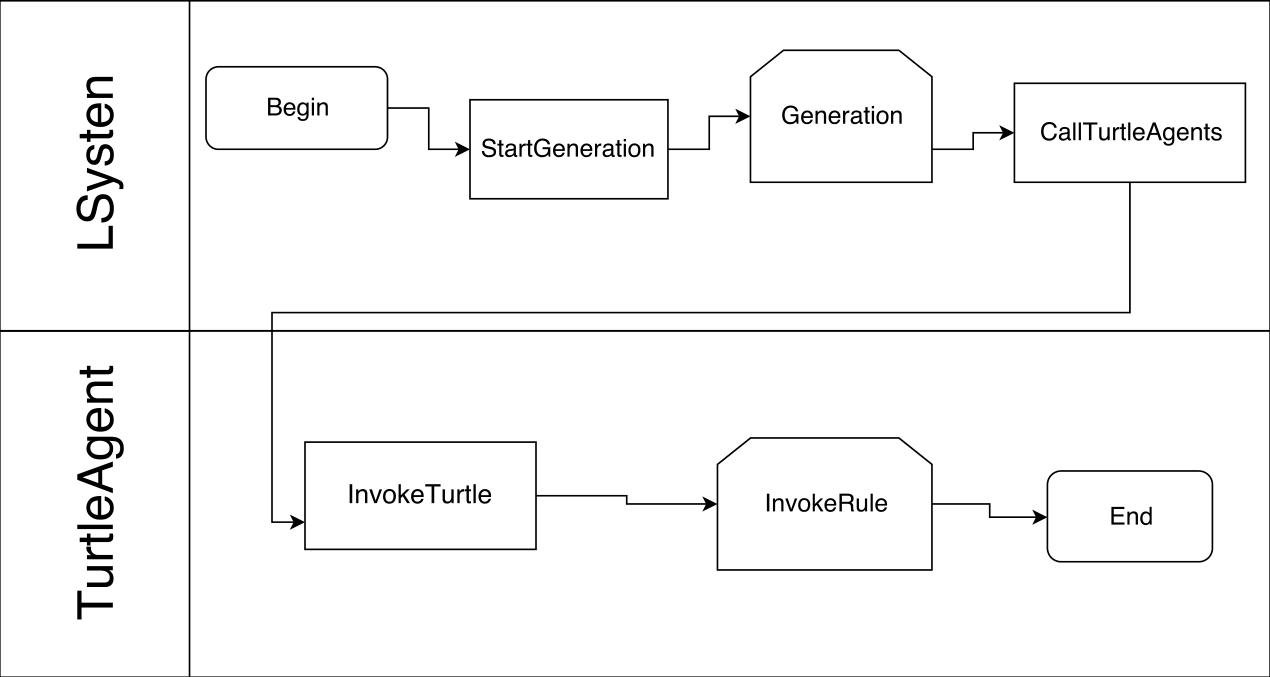
\includegraphics[width=0.4\textwidth]{LSystemFlow}
	\caption{Fluxo da ferramenta LSystem2Unity}
	\label{LSystemFlow}
\end{figure}

\subsection{Interface da ferramenta}
O componente principal para a geração das estruturas esta no monobehaviour LSystem demostrado na figura \ref{LSystemComponent}, nele tem as propriedades principais, além do campo para por uma lista de regras de substituição.

\begin{figure}[!h]
	\centering
	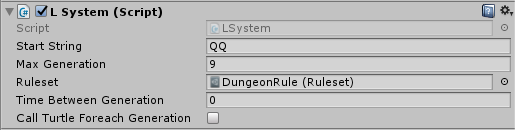
\includegraphics[width=0.4\textwidth]{LSystemComponent}
	\caption{Interface do componente LSystem}
	\label{LSystemComponent}
\end{figure}

A figura \ref{LRuleSet} apresenta a interface de Ruleset já customizada, aonde o usuário pode ver com mais facilidade os símbolos que vão ser trocados, além de botões para adicionar e remover novas regras.
\begin{figure}[!h]
	\centering
	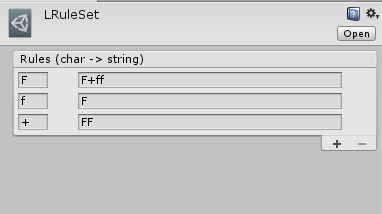
\includegraphics[width=0.4\textwidth]{LRuleEditor}
	\caption{Interface de Ruleset}
	\label{LRuleSet}
\end{figure}

 A interface do componente TurtleAgent possui a mesma semelhança, mas para facilitar a leitura do componente, há uma funcionalidade de mostrar o conteúdo presente na lista somente quando o item for selecionado, isso é demostrado nas figuras \ref{TurtleAgentWithout} e \ref{TurtleAgentSelect}, com o item não selecionado e selecionado respectivamente.

\begin{figure}[!h]
	\centering
	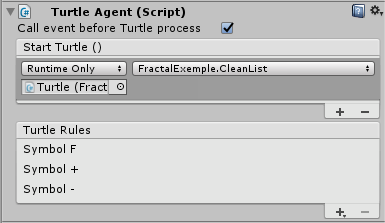
\includegraphics[width=0.3\textwidth]{TurtleAgentInspectorNoSelected}
	\caption{Interface de TurtleAgent sem item selecionado}
	\label{TurtleAgentWithout}
\end{figure}

\begin{figure}[!h]
	\centering
	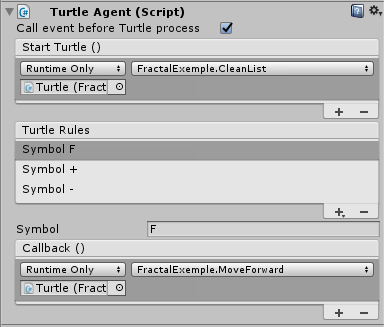
\includegraphics[width=0.3\textwidth]{TurtleAgentInspectorSelected}
	\caption{Interface de TurtleAgent com item selecionado}
	\label{TurtleAgentSelect}
\end{figure}
\section{Exemplos}
Foi criado um gerador de cenários 2D para realizar os testes do plugin, o exemplo em questão foi rodado no editor do Unity 2017.1 em um computador com processador Intel Core i5-3470S de 2.90GHz, com 8Gb de ram. Durante o teste foi analisado o tempo de execução do processo durante as gerações.
\label{cenarioSection}
Foi feito um criador de cenários que monta um mapa distribuindo os pisos pelo cenário, é utilizado as seguintes regras da tabela \ref{cenárioRules} na geração do cenário.

\begin{table}[]
	\centering
	\begin{tabular}{ll}
		Q $\Rightarrow$   & QQ{[}Q \\ 
		{[} $\Rightarrow$ & +QQ{]} \\ 
		{]} $\Rightarrow$ & QQ+QQ  \\ 
	\end{tabular}
	\caption{Conjunto de regras do L-System}
	\label{cenárioRules}
\end{table}

Ao finalizar o TurtleAgent faz a leitura da estrutura gerada pelo LSystem e monta o mapa usando como referencia a tabela \ref{cenárioTurtle}. O cenário obtido com o axioma inicial de "QQ" com 8 gerações pode ser visto na figura \ref{cenário8Gen} e na figura \ref{cenário9Gen} apresenta um cenário gerado em 6 iterações com o axioma inicial "Q+".
\begin{table}[]
	\centering
	\begin{tabular}{ll}
		Q $\Rightarrow$   & Gera um quarto.                              \\
		+  $\Rightarrow$  & Gira a direita a um ângulo de 90º.            \\
		-  $\Rightarrow$  & Gira a esquerda a um ângulo de 90º.           \\
		{[}  $\Rightarrow$ & Salva a posição e rotação atual.             \\
		{]}  $\Rightarrow$ & Volta para a ultima posição e rotação salva.
	\end{tabular}
	\caption{Regras de interpretação do TurtleAgent.}
	\label{cenárioTurtle}
\end{table}

\begin{figure}[!h]
	\centering
	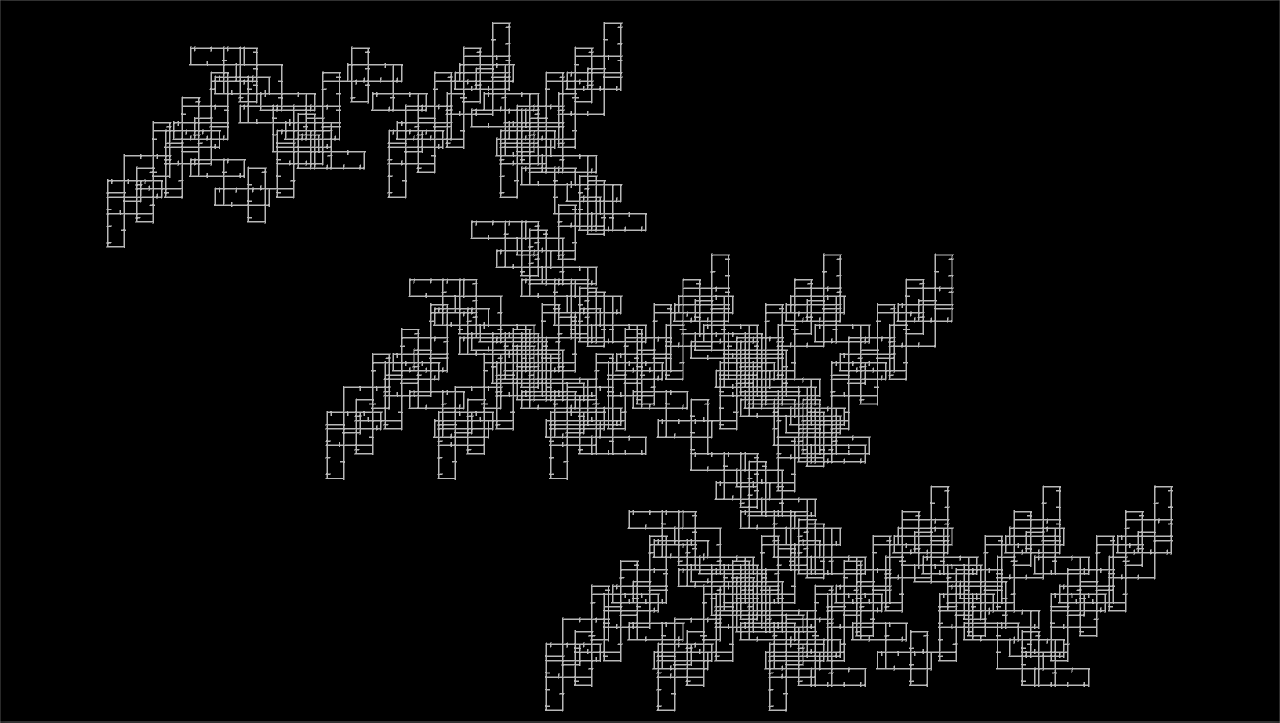
\includegraphics[width=0.4\textwidth]{Cenario2-Gen8}
	\caption{Cenário produzido na 8ª geração.}
	\label{cenário8Gen}
\end{figure}

\begin{figure}[!h]
	\centering
	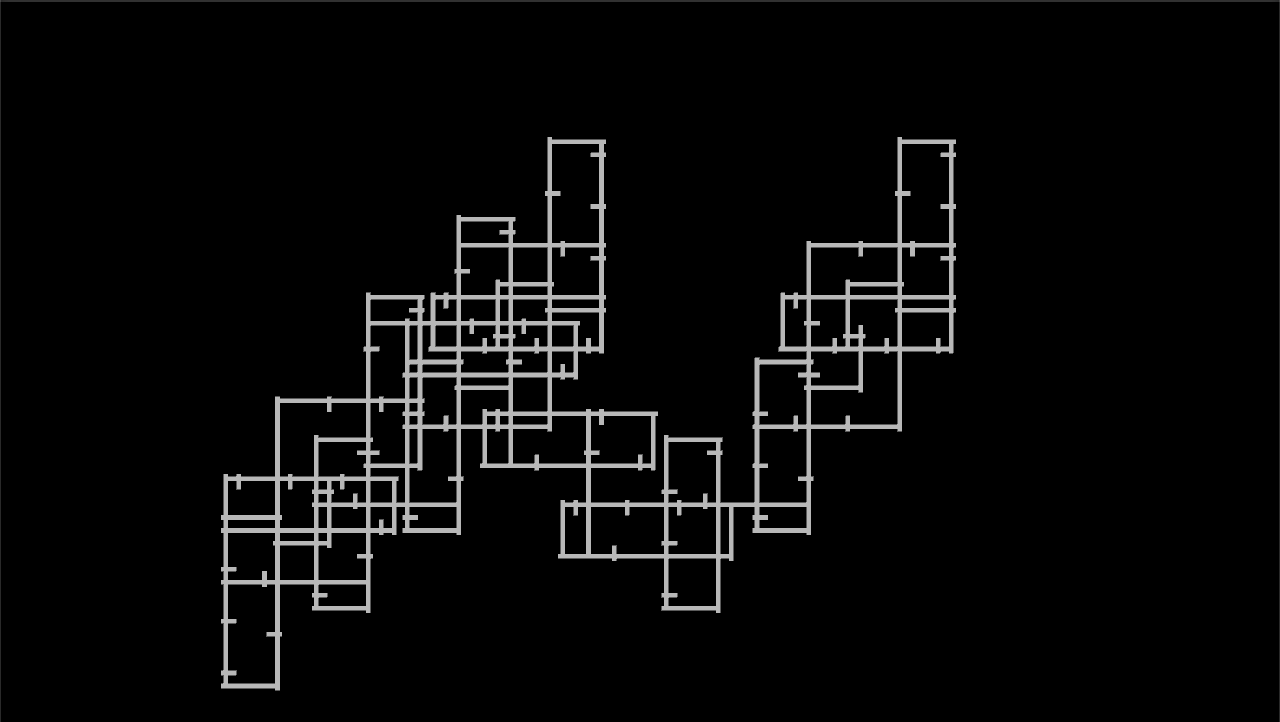
\includegraphics[width=0.4\textwidth]{Cenario3Q+-Gen6}
	\caption{Cenário produzido na 6ª geração.}
	\label{cenário9Gen}
\end{figure}

É fácil a configuração e implementação das regras usando o editor, o sistema de reescrita é bom para geração de cenários, mas necessita de algoritmos mais especializados para geração mais complexas.

\subsection{Desempenho}
Utilizando as regras de reescrita da tabela \ref{cenárioRules} na seção \ref{cenarioSection}, foi medido o tempo de execução por comprimento do axioma, definindo 15 como o numero máximo de gerações os resultados estão presentes na tabela  \ref{axiomaTempoTabela}.

\begin{table}[!h]
	\centering
	\begin{tabular}{|c|c|}
		\hline
		\textbf{Comprimento do Axioma} & \textbf{Tempo(s)} \\ \hline
		32                             & 0,0000142         \\ \hline
		124                            & 0,0000293         \\ \hline
		472                            & 0,0000917         \\ \hline
		25980                          & 0,0046719         \\ \hline
		98792                          & 0,0176053         \\ \hline
		1428512                        & 0,2621754         \\ \hline
		20655832                       & 03,7396957        \\ \hline
		78545636                       & 14,1387742        \\ \hline
		298676752*                     & 29,6070016        \\ \hline
	\end{tabular}
	\caption{Tabela com o tamanho do axioma e o tempo para ser processado em segundos. *Geração incompleta}
	\label{axiomaTempoTabela}
\end{table}

A ultima geração chegou a capacidade máxima suportada pelo stringbuilder, sua geração incompleta levou em torno de 34 segundos para ser realizada.

A figura \ref{profilerCPU} apresenta a tela do profiler na Unity sobre o uso da cpu durante os processos, aonde verifica-se a instabilidade de fps entre os processamentos, já na figura \ref{profilerMemoria} tem o uso de memoria da ferramenta durante o processamento dos axiomas, chegando até 4,80 Gb alocados na memoria.
\begin{figure}[]
	\centering
	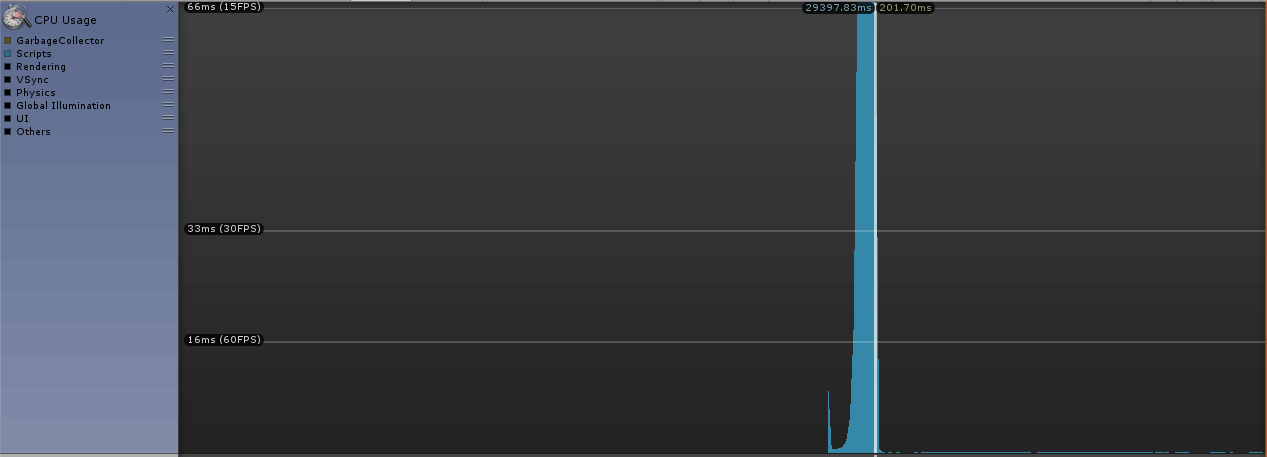
\includegraphics[width=0.45\textwidth]{Cenario-Profiler-15Gen-CPU}
	\caption{Profiler da Unity com o uso da cpu.}
	\label{profilerCPU}
\end{figure}

\begin{figure}[]
	\centering
	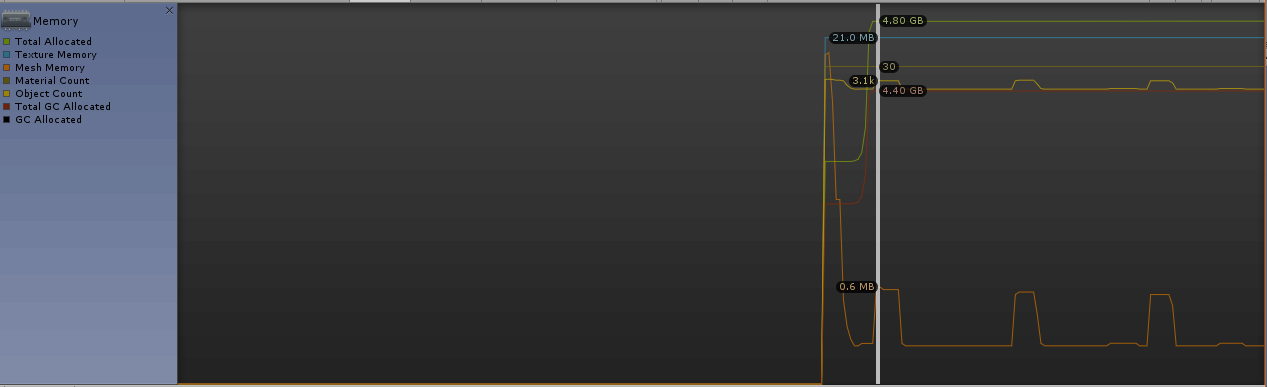
\includegraphics[width=0.45\textwidth]{Cenario-Profiler-15Gen-Memoria}
	\caption{Profiler da Unity do uso de memoria.}
	\label{profilerMemoria}
\end{figure}
\section{Conclusão}
No artigo foi descrito o desenvolvimento e a implementação do L-System no Unity atráves do asset denominado de LSystem2Unity, no qual dá aos desenvolvedores a possibilidade de aplicar o L-Sistemas em seus projetos com maior facilidade, desde criação de regras para o l-sistema, quanto ao interpretador TurtleAgent.

Durante o desenvolvimento, percebeu-se que é simples de utilizar, podendo protótipar rapidamente uma geração, definindo somente as regras de reescrita do LSystem e fazendo a ligação dos eventos no TurtleAgent com os métodos a serem utilizados pelo desenvolvedor.

A ferramenta ainda possui certas limitações referente a quantidade de tipos de regras a serem utilizados, possuindo somente um sistema implementado, diminuindo as opções de diversificação aos desenvolvedores.

\section{Trabalhos Futuros}
É planejado dar a ferramenta mais estruturas de regras, dando aos desenvolvedores uma maior variedade de opções nos desenvolvimentos de assets em seus jogos. Trazer mais funcionalidades ao editor do Unity, melhorando a utilização da ferramenta. Um ponto essencial é melhorar a performance, diminuindo os recursos de memória e demora de processamento das gerações em grande cadeias de caracteres.

A possibilidade da implementação para a produção de estruturas no editor, deixando os designers criarem conteúdos para os jogos, podendo optimizar e editar os elementos já produzidos.

% use section* for acknowledgement
\section*{Agradecimentos}
Agradeço aos meus pais, Miguel Ângelo e Perenice Socorro, além a minha irmã Ana Virgínia por terem criado diversas oportunidades para mim e por sempre estarem me acompanhando na minha vivencia me apoiando, dando conselhos.

Ao meu professor e orientador Adriano Gil no qual me criou o interesse pelos campos de PCG e IA em jogos. Aos meus amigos da época de ensino médio e os que construir durante o curso, os quais me acompanharam durante esse anos, além dos professores Rodrigo Braga, Rafael Lima, Raphael Maquiné e André Machado.

A Vivian Fonseca por sempre me apoiar e a me incentivar no meu desenvolvimento profissional e acadêmico. A Universidade do Estado do Amazonas por ter proporcionado o curso Tecnólogo em Jogos Digitais e ao coordenador do curso Cleto Leal.

\bibliographystyle{IEEEtran}
\bibliography{refs}

\end{document}


